\subsection*{Abstract Syntax Tree}\label{sec:AST}
The parser creates a parse tree which contains a node for each production of \gls{gamble}'s grammar.
This tree contains unneeded information, which makes it difficult to traverse the tree and check for the semantics of \gls{gamble}.
Therefore the tree will be transformed into what is called an \acrfull{ast}.
The \acrshort{ast} should be able to express the same source code as the parsetree, and therefore one should be able to make a pretty printer from it.
A pretty printer, is a program which takes the \acrshort{ast} as input, and outputs the original source code i.e. without loss of information.
If this is possible to implement such a pretty printer the \acrshort{ast} contains all possible information from the source code.
A transformation from a parse tree to an \acrshort{ast}, on the declaration: \texttt{int a = 5;} (using the grammar of \gls{gamble}) can be seen on \myref{image:AST}

\begin{figure}
		\centering
	 	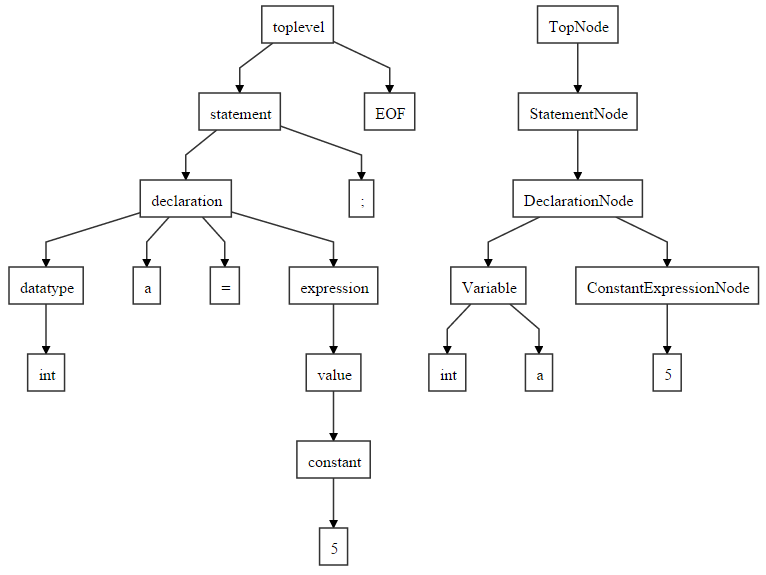
\includegraphics[width=0.8\linewidth]{figures/Trees/AST.PNG}
		\caption{The tree on the left is the parse tree, and the tree on the right is the AST, which still contains all the information from the parse tree.}\label{image:AST}
\end{figure}

The parse tree is generated using a parser produced by compiling the grammar with ANTLR, which means we cannot decide which information is contained on the nodes of the tree.
The nodes of the \acrshort{ast} can therefore be made to contain information for type and scope checking, which helps in the contextual analysis phase.
All that is needed to make this transformation, is to make classes for all the nodes of the \acrshort{ast}, a way to traverse the parsetree, and creating instances of the \acrshort{ast} nodes as the traversal is ongoing.



